\documentclass{sintefbeamer}
\usepackage{amsfonts,amsmath,oldgerm}
%\usepackage{sidecap}
\usepackage{bm}
\usepackage{subfig}
\usepackage{stmaryrd}%\mapsfrom
\usepackage{graphbox} % allows includegraphics[align=c]

\newcommand{\mr}{\mathrm}
\newcommand{\mc}{\mathcal}
\let\SSS\S
\renewcommand{\S}{^\mr{S}}
\newcommand{\ii}{\mr{i}\,}
\newcommand{\ee}{\mr{e}}
%\newcommand{\phit}{\psi}
\newcommand{\phit}{\tilde\phi}
\newcommand{\br}[3]{\left#1#2\right#3}
\let\underscore\_
\renewcommand{\_}[1]{_\mr{#1}}
\newcommand{\oo}[1]{^{(#1)}}
\let\Re\relax
\let\Im\relax
\DeclareMathOperator\Re{Re}
\DeclareMathOperator\Im{Im}
\newcommand{\w}{w}
\newcommand{\ww}{\omega}
\newcommand{\zmap}{f}
\newcommand{\iJac}{|\zmap_\zz|^{-2}}


\newcommand{\bU}{\bm U}
\newcommand{\z}{z}
\newcommand{\x}{x}
\newcommand{\y}{y}
\newcommand{\zz}{\zeta}
\newcommand{\xx}{\xi}
\newcommand{\yy}{\sigma}
\newcommand{\h}{\hat}
\newcommand{\rbr}[1]{\left(#1\right)}
\newcommand{\sbr}[1]{\left[#1\right]}
\newcommand{\cbr}[1]{\left\{#1\right\}}

\newcommand{\testcolor}[1]{\colorbox{#1}{\textcolor{#1}{test}} \texttt{#1}}
\usefonttheme[onlymath]{serif}
\newcommand{\hrefcol}[2]{\textcolor{cyan}{\href{#1}{#2}}}

\title{Extensions for the Higher Order Spectral method, and st{\o}ff}
%\subtitle{}
\author{\href{mailto:andreas.akselsen@sintef.no}{Andreas Holm Akselsen}}
\date{April 15, 2021}
%\titlebackground{} % removes background

% separate section slide
\AtBeginSection[]{
  \begin{frame}
  \vfill
  \centering
  \begin{beamercolorbox}[sep=8pt,center,shadow=true,rounded=true]{title}
    \usebeamerfont{title}\insertsectionhead\par%
  \end{beamercolorbox}
  \vfill
  \end{frame}
}

\begin{document}
\maketitle

\newcommand {\framedgraphic}[2] {
    \begin{frame}{#1}
        \begin{center}
            \includegraphics[width=\textwidth,height=0.8\textheight,keepaspectratio]{#2}
        \end{center}
    \end{frame}
}


\begin{frame}{Interests related to OSC}
\vspace{-.5cm}
\begin{minipage}{.25\framewidth}
\small
\begin{block}{Wave quality concerns}
	\begin{itemize}
		\item Wavemaker
		\item Basin walls
		\item Bathymetry
		\item Wave-current interaction
		\item Beaches
	\end{itemize}
	\end{block}
\end{minipage}
\hfill
\begin{minipage}{.7\framewidth}
\small
	\begin{block}{Development}
	\begin{itemize}
		\item 2nd \& 3rd order wavemaker perturbation theory
		\item 2nd order wavemaker theory for multi-hinged wavemakers
		\item Extension of HOS for exact representation of wavemeakers (ongoing)
		\item Linear theory for basin geometry
		\item Linear and 2nd order theory for discontinuous depth transitions
		\item Extension of HOS for abrupt or gradual depth transitions
		\item Extension of HOS for potential current flow		
		\item Beach reflection experiments
	\end{itemize}
	\end{block}
\end{minipage}
\end{frame}

\begin{frame}{The Higher Order Spectral method, in one slide}
\vspace{-1cm}
\begin{center}
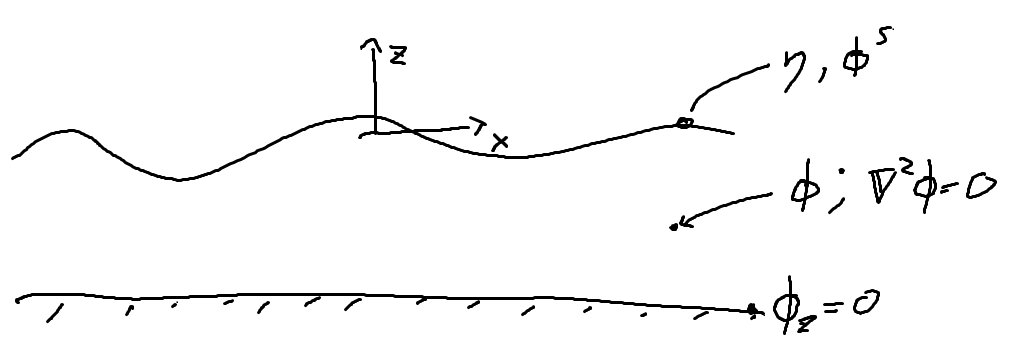
\includegraphics[width=.5\framewidth]{HOS1.png}
\end{center}

Body of fluid represented analytically:
\begin{align*}
\nabla^2\phi = 0;\qquad  \phi(\bm r,z,t) = \sum_{j=1}^N \hat\phi_j(t) \frac{\cosh k_j(z+h)}{\cosh k_j h} \ee^{\ii \bm r \cdot \bm k}.
\end{align*}

We solve only the equations for the free surface 
\begin{align*}
\eta_t &=   - \nabla\eta\cdot\nabla\phi\S     + \big(1+|\nabla\eta|^2\big)\w, %(\Phi_z)_{z=\eta} 
\\
\phi\S_t &= - \frac12\big|\nabla\phi\S|^2 + \frac12\big(1+|\nabla\eta|^2\big)\w^2 - g\eta.
\end{align*}
with an ODE solver and match the modes $\hat\phi_j(t) $ to the surface potential $\phi\S(\bm r,t)$.
\end{frame}


\section{Representing currents (potential flow) in HOS}

\begin{frame}{Currents in HOS}{Example: Waves propagating over a horizontal line vortex}
\centering
\vspace{-.25cm}
\begin{minipage}{.5\framewidth}
%\resizebox{3cm}{!}{
\scriptsize
	\begin{align*}
\eta_t &=   - \nabla\eta\cdot\nabla\phi\S  - \nabla\eta\cdot\bU + W  + \big(1+|\nabla\eta|^2\big)\w
\\
\phi\S_t &= -\Phi_t\big|_{z=\eta} - \frac12\big|\nabla\phi\S +\bU\big|^2 + \frac12\big(1+|\nabla\eta|^2\big)\w^2 - g\eta
\end{align*}
\normalsize 
  %}
\includegraphics[width=\columnwidth]{../doc/figures/flowField_vortex.pdf}%
\end{minipage}%
%\hfill
\includegraphics[width=.5\framewidth,align=c]{../doc/figures/waveField_vortex.pdf}%
\end{frame}




\begin{frame}{Currents in HOS}{Examining the effect of recirculation from the OB current system}
\centering
\vspace{-.25cm}
\begin{minipage}{.5\framewidth}
\includegraphics[width=\columnwidth]{C:/gits/SFo_gitHOS/hosm-nwt2d/basinSpec/novortex_flipLinear_Lh50x15_nx256nk512_patchPos8xm1p8x0x0_Uj0_posZ0.pdf}\\
\includegraphics[width=\columnwidth]{C:/gits/SFo_gitHOS/hosm-nwt2d/basinSpec//flipLinear_Lh50x15_nx256nk512_dimVort15x3p5_Uj0p55_posZ0.pdf}%
\end{minipage}%
%\hfill
\includegraphics[width=.5\framewidth,align=c]{C:/gits/SFo_gitHOS/hosm-nwt2d/results/merged/snapCompare_T1p5CM2.pdf}\\
%$T=1.5$\,s, double current strength.
\end{frame}



%%%%%%%%%%%%%%%%%%%%%%%%%%%%%%%%%%%%%%%%%%%%%%%

\section{Accounting for abrupt  bathymetry variation with conformal mapping}



\begin{frame}{Conformal mapping}
\centering
	%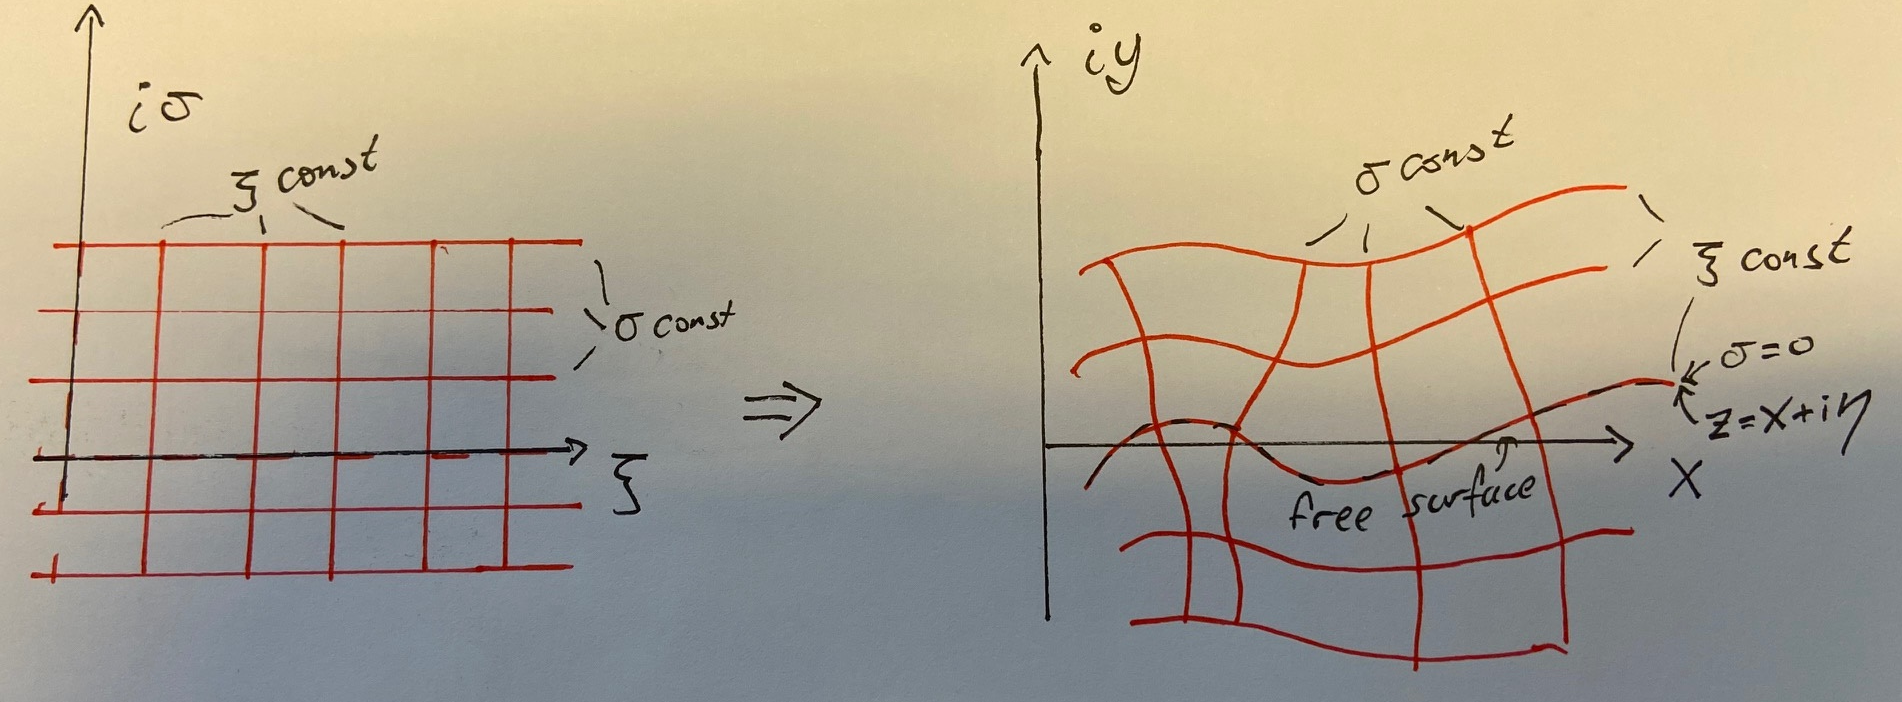
\includegraphics[width=.5\framewidth]{map.png}
	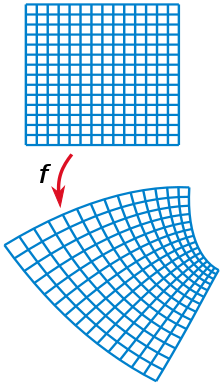
\includegraphics[width=.22\framewidth]{220px-Conformal_map.svg.png}
	\hspace{2cm}
	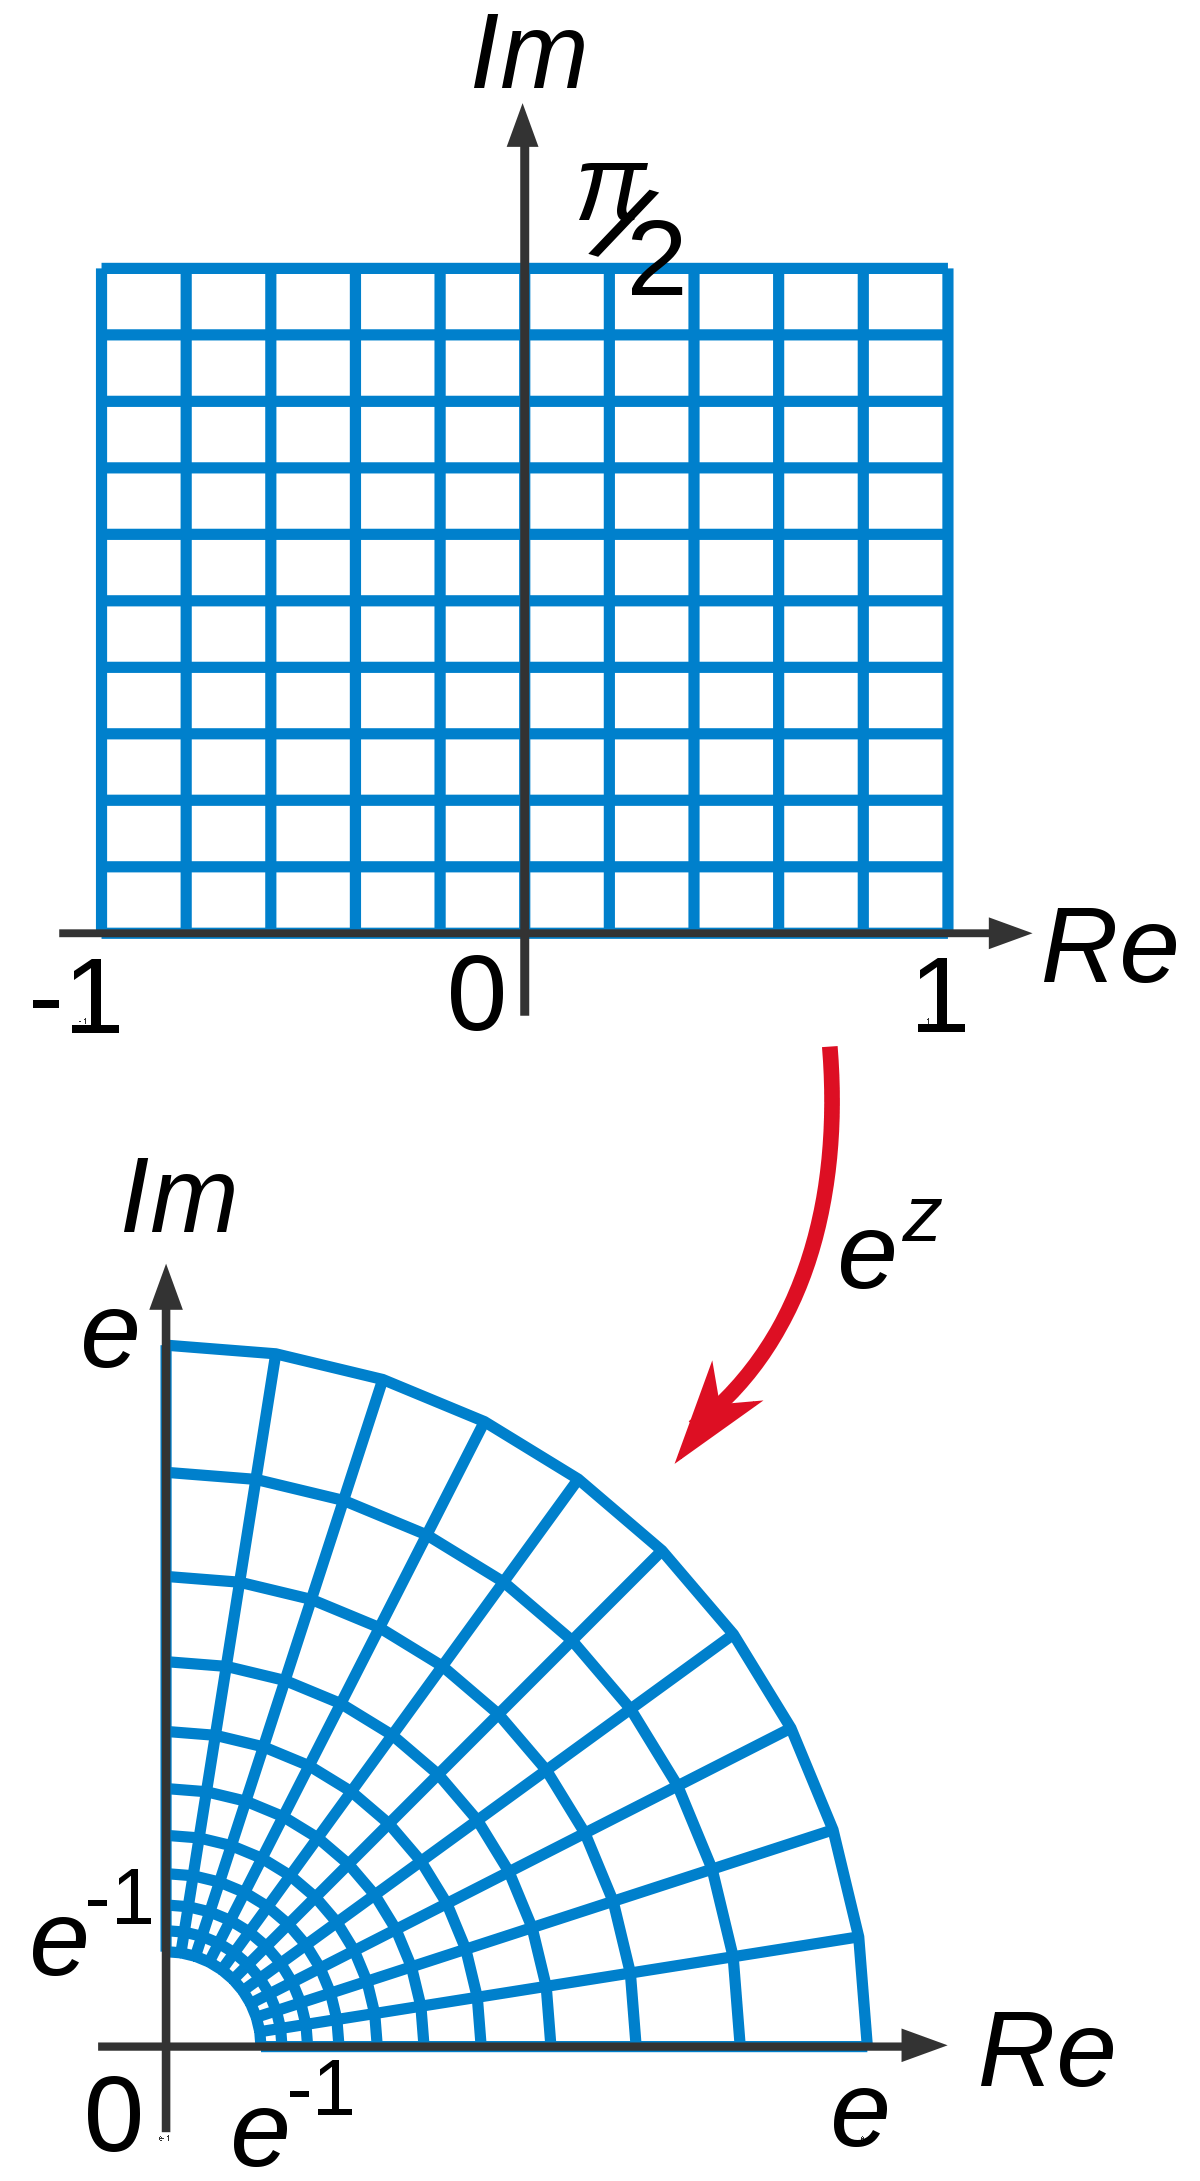
\includegraphics[width=.22\framewidth]{1200px-Biholomorphism_illustration.svg.png}\\
	
	Analytic representation of $\phi$ remains valid in all planes.
\end{frame}

%%%%%%%%%%%%%%%%%%%%%%%%%%%%%%%%%%%%%%%%%%%%%%%%%


\begin{frame}{Conformally mapped bathymetry}{Step depth transitions}
\vspace{-.5cm}
%\centering
%\begin{figure}%
%\subfloat[$\z$-plane]{\includegraphics[width=.5\columnwidth]{../conformalMapping/conformalBathymetry/CCMei_step.pdf}}%
%\subfloat[$\zz$-plane]{\includegraphics[width=.5\columnwidth]{../conformalMapping/conformalBathymetry/CCMei_step_inv.pdf}}%
%%\caption{}
%\end{figure}
%\begin{tabular}{ccc}
\parbox[c]{.45\framewidth}{\centering
\includegraphics[width=.45\framewidth]{../conformalMapping/conformalBathymetry/CCMei_step_inv.pdf}
$\zz$-plane
}
\hfill$\rightarrow$ \hfill
\parbox[c]{.45\framewidth}{\centering
\includegraphics[width=.45\framewidth]{../conformalMapping/conformalBathymetry/CCMei_step.pdf}
$\z$-plane
}
%\end{tabular}
%\vspace{.5cm}

\footnotesize
Analytical map for step transition:
\begin{align*}
\lambda &= \exp(\zz),&
\tau &= \sqrt{\frac{\lambda+c^2}{\lambda+1} },&
z &\mapsfrom f(\zz) = -\ii H\_s +\frac{H\_d}{\pi}\left[\frac1c \ln^+\frac{\tau-c}{\tau+c} - \ln\frac{\tau-1}{\tau+1}\right].
\end{align*}%
Surface equations in the $\zz$-plane:
\begin{align*}
\eta_t &= \iJac\sbr{\varphi_\yy\rbr{1+\eta_\xx^2}-\varphi\S_\xx} + \eta_\xx \Re\rbr{\frac{\zmap_t}{\zmap_\zz}}-\Im\rbr{\frac{\zmap_t}{\zmap_\zz}},\\
\varphi\S_t &= - \frac12\iJac\sbr{\rbr{\varphi\S_\xx}^2-\rbr{1+\eta_\xx^2}\varphi_\yy^2} - gh + \varphi\S_\xx \Re\rbr{ \frac{\zmap_t}{\zmap_\zz}}.
\end{align*}

\end{frame}

%%%%%%%%%%%%%%%%%%%%%%%%%%%%%%%%%%%%%%%%%%%


\begin{frame}{Conformally mapped bathymetry}{Slope depth transitions}
\vspace{-1cm}
\small
\begin{equation*}
f'(\zz) \mapsfrom K \prod_{j=1}^{N_\angle} \rbr{\frac{\exp(\zz-\xi^\angle_j)+1}{\exp(\zz-\xx^\angle_j) + (H_{j+1}/H_j)^{\pi/\theta_j}}}^{\theta_j/\pi}
\end{equation*}
\normalsize

\includegraphics[width=.45\framewidth,align=c]{../conformalMapping/conformalBathymetry/SCnumStep2x45deg_zz.pdf}
$\rightarrow$
\includegraphics[width=.45\framewidth,align=c]{../conformalMapping/conformalBathymetry/SCnumStep2x45deg_z.pdf}
\\


\includegraphics[width=.45\framewidth,align=c]{../conformalMapping/conformalBathymetry/SCnumStepMulti_zz.pdf}
$\rightarrow$
\includegraphics[width=.45\framewidth,align=c]{../conformalMapping/conformalBathymetry/SCnumStepMulti_z.pdf}

\end{frame}

%%%%%%%%%%%%%%%%%%%%%%%%%%

\begin{frame}{Comparing ramp slopes}
\begin{figure}%
\subfloat[$\theta=45$\textdegree]{\includegraphics[width=.33\framewidth]{../HOS_bathymetry/figures/map/mapZoom_SSGW_ka0p05_H1p00_0p50_nH2_ang1_0p5_Nw60.pdf}}%
\subfloat[$\theta=9$\textdegree]{\includegraphics[width=.33\framewidth]{../HOS_bathymetry/figures/map/mapZoom_SSGW_ka0p05_H1p00_0p50_nH2_ang1_0p1_Nw60.pdf}}%
\subfloat[$\theta=4.5$\textdegree]{\includegraphics[width=.33\framewidth]{../HOS_bathymetry/figures/map/mapZoom_SSGW_ka0p05_H1p00_0p50_nH2_ang1_0p05_Nw60.pdf}}%
\caption{Depth transition maps}
\end{figure}
\end{frame}


\begin{frame}{Step bathymetry, $H\_s/H\_d = 0.50$.}
\centering 
\vspace{-1cm}
\includegraphics[width=.75\framewidth]{../HOS_bathymetry/figures/logstrip_SSGW_ka0p05_M5_H1p00_0p50_Nw60_dt5T_nx3840_pad0_ikCutInf_Md0p5_r0p25.pdf}%
\end{frame}

\begin{frame}{45\textdegree{} slope depth transition.}
\centering
\vspace{-1cm}
 \includegraphics[width=.75\framewidth]{../HOS_bathymetry/figures/SSGW_ka0p05_M5_H1p00_0p50_nH2_ang1_0p5_Nw60_dt5T_nx3840_pad0_ikCutInf_Md0p5_r0p25.pdf}%
%\caption{Surface elevation, $(ka)_0 = 0.05$, $(kH)_0 = 1.00$ ($H\_d=1.0$\,m corresponds to $T\approx2.30$\,s); single slope with $\theta=\pi/4$; $H\_s/H\_d = 0.5$. Dashed lines indicate $\x$-location of slope transition beginning and end.}%
\end{frame}

\begin{frame}{9\textdegree{} slope depth transition.}
\centering
\vspace{-1cm}
 \includegraphics[width=.75\framewidth]{../HOS_bathymetry/figures/SSGW_ka0p05_M5_H1p00_0p50_nH2_ang1_0p1_Nw60_dt5T_nx3840_pad0_ikCutInf_Md0p5_r0p25.pdf}%
%\caption{Similar to \autoref{fig:res:slope1}, but with $\theta=\pi/20$.}%
\end{frame}

\begin{frame}{4.5 \textdegree{} slope depth transition.}
\centering
\vspace{-1cm}
 \includegraphics[width=.75\framewidth]{../HOS_bathymetry/figures/SSGW_ka0p05_M5_H1p00_0p50_nH2_ang1_0p05_Nw60_dt5T_nx3840_pad0_ikCutInf_Md0p5_r0p25.pdf}%
%\caption{Similar to \autoref{fig:res:slope1}, but with $\theta=\pi/40$.}%
\end{frame}


\begin{frame}{Testing effect of beach extensions}
	\begin{figure}[H]
		\vspace{-1cm}
		\begin{minipage}[c]{.45\textwidth}\centering
		\includegraphics[width=\textwidth,align=c]{../conformalMapping/conformalBathymetry/beachRamp_h10D4th90_z.pdf}\\
		No beach extension
		\end{minipage}%
		\hfill
		\begin{minipage}[c]{.5\textwidth}\centering
			\includegraphics[width=1\textwidth]{../conformalMapping/conformalBathymetry/beachRamp_h10D4th45_z.pdf}\\
			$\theta=45$\textdegree{} beach extension.\\
			\includegraphics[width=1\textwidth]{../conformalMapping/conformalBathymetry/beachRamp_h10D4th30_z.pdf}\label{fig:map:30}\\
			$\theta=30$\textdegree{} beach extension.
		\end{minipage}
%		\subfloat[$\zz$-plane of map in \protect\subref{fig:map:30} ]{\includegraphics[width=.7\textwidth]{../conformalMapping/conformalBathymetry/beachRamp_h10D4th30_zz.pdf}}%
%		\caption{Bathymetries and conformal maps. Dashed line indicates the Lader tank beach profile $\y=-D(\x/L)^2$; $D/L=0.353$.}
		\label{fig:maps}
	\end{figure}
\end{frame}


\begin{frame}{	No beach extension, 2.50 second period.}
	\centering
	\vspace{-5mm}
	\includegraphics[width=.7\framewidth]{../HOS_bathymetry/figures/beach_SSGW_T2p50_ka0p05_M5_H10p00_2p00_theta90_Nw60_dt5T_nx3840_pad0_ikCutInf_Md0p5_r0p25_a10p0777_aRef0p00314.pdf}\\
\end{frame}

\begin{frame}{	$\theta=45$\textdegree{} beach extension, 2.50 second period.}
	\centering
	\vspace{-5mm}
	\includegraphics[width=.7\framewidth]{../HOS_bathymetry/figures/beach_SSGW_T2p50_ka0p05_M5_H10p00_8p30_4p90_2p00_theta90_180_45_Nw60_dt5T_nx3840_pad0_ikCutInf_Md0p5_r0p25_a10p0777_aRef0p00155.pdf}\\
\end{frame}

\begin{frame}{$\theta=30$\textdegree{} beach extension, 2.50 second period.}
\centering
\vspace{-5mm}
	\includegraphics[width=.7\framewidth]{../HOS_bathymetry/figures/beach_SSGW_T2p50_ka0p05_M5_H10p00_9p10_4p60_2p00_theta90_180_30_Nw60_dt5T_nx3840_pad0_ikCutInf_Md0p5_r0p25_a10p0777_aRef0p00149.pdf}\\
\end{frame}






%%%%%%%%%%%%%%%%%%%%%%%%%%%%


\begin{frame}{Power spectra in front and after depth transition}
\vspace{-1cm}
\scriptsize
	\begin{figure}[h!ptb]%
	\centering
	\subfloat[Bathymetries]{
		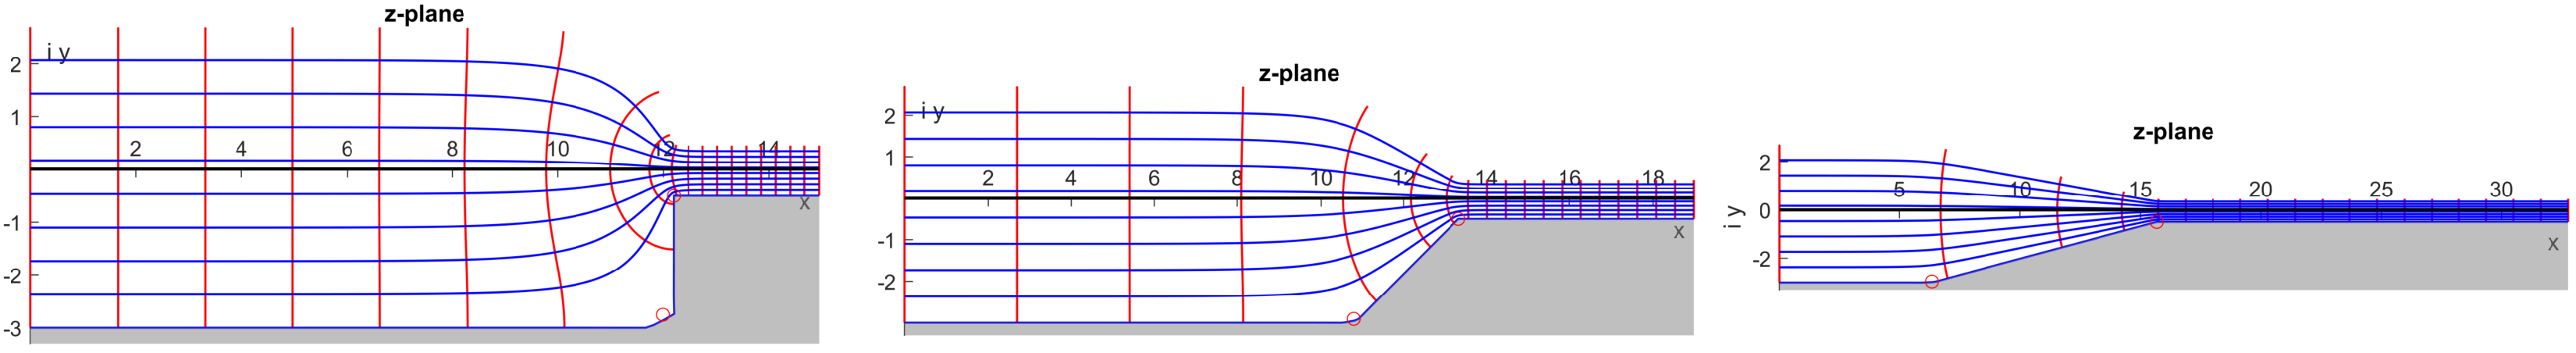
\includegraphics[width=.75\columnwidth]{./zmapsCrop.png}
	%\includegraphics[width=.2\columnwidth]{../HOS_bathymetry/figures/map/mapZoom_82100_linear_ka0_H3p00_0p50_theta90_Nw1.pdf}
	%\includegraphics[width=.2\columnwidth]{../HOS_bathymetry/figures/map/mapZoom_82000_linear_ka0_H3p00_0p50_theta45_Nw1.pdf}
	%\includegraphics[width=.2\columnwidth]{../HOS_bathymetry/figures/map/mapZoom_82100_linear_ka0_H3p00_0p50_theta15_Nw1.pdf}
	}\\[-4mm]%
	\subfloat[$x=5.0$\,m.]{
	\includegraphics[width=.28\columnwidth]{../HOS_bathymetry/figures/powerSpec/82100/x_wp5.pdf}}%
	\subfloat[$x=10.0$\,m.]{
	\includegraphics[width=.28\columnwidth]{../HOS_bathymetry/figures/powerSpec/82100/x_wp10.pdf}}\\[-4mm]
	\subfloat[$x=15.0$\,m.]{
	\includegraphics[width=.28\columnwidth]{../HOS_bathymetry/figures/powerSpec/82100/x_wp15.pdf}}%
	\subfloat[$x=20.0$\,m.]{
	\includegraphics[width=.28\columnwidth]{../HOS_bathymetry/figures/powerSpec/82100/x_wp20.pdf}}%
	\subfloat[$x=25.0$\,m.]{
	\includegraphics[width=.28\columnwidth]{../HOS_bathymetry/figures/powerSpec/82100/x_wp25.pdf}}%
	\caption{Power spectra measured at various locations, comparing transitional ramps.
	%Depth transition from 3.0 to 0.5 meters.
	%$T\_p=2.5$\,s, $H\_s=0.125$\,m.
	}
	%\label{fig:S}%
	\end{figure}
\end{frame}

\begin{frame}{Flat bottom reference}
%\vspace{-1cm}
\scriptsize
\begin{figure}[h!ptb]%
\centering
\subfloat[$x=5.0$\,m.]{
\includegraphics[width=.28\columnwidth]{../HOS_bathymetry/figures/powerSpec/82100_flatOnly/x_wp5.pdf}}%
\subfloat[$x=10.0$\,m.]{
\includegraphics[width=.28\columnwidth]{../HOS_bathymetry/figures/powerSpec/82100_flatOnly/x_wp10.pdf}}\\[-4mm]
\subfloat[$x=15.0$\,m.]{
\includegraphics[width=.28\columnwidth]{../HOS_bathymetry/figures/powerSpec/82100_flatOnly/x_wp15.pdf}}%
\subfloat[$x=20.0$\,m.]{
\includegraphics[width=.28\columnwidth]{../HOS_bathymetry/figures/powerSpec/82100_flatOnly/x_wp20.pdf}}%
\subfloat[$x=25.0$\,m.]{
\includegraphics[width=.28\columnwidth]{../HOS_bathymetry/figures/powerSpec/82100_flatOnly/x_wp25.pdf}}%
\caption{Power spectra measured at various locations, flat bed at 0.5 meters depth.}
\label{fig:S}%
\end{figure}
\end{frame}








%%%%%%%%%%%%%%%%%%%%%%%%%%%%%%%%%%%%%%%%%%%%%%%%%%%%%%

\section{Conformally mapping the free surface itself}

\begin{frame}{Conformally mapped free surface}
\centering
\vspace{-1cm}
\small
\begin{align*}
\z \mapsfrom f(\zz) &= \sum_{j=-M}^M \h f_j \,\frac{\ee^{\ii k_j(\zz+\ii H)}}{\cosh(k_j H)}
&
\z \mapsfrom f(\zz) &= \sum_{j=-M}^M \h f_j \,\frac{-\ee^{\ii k_j(\zz+\ii H)}}{\sinh(k_j H)}.
 \end{align*}%
\normalsize

\includegraphics[width=.8\framewidth]{../HOS_old/conformalHOS/figures/imagedecayingConformalka0p2_M5_h1p00_Nw1_dt0p25T_nx512.pdf}%
\end{frame}

\begin{frame}{Conformally mapped free surface}
	\centering
%\vspace{-.5cm}
\includegraphics[width=.6\framewidth]{../HOS_ChalikovTaylor_current/figures/rounded2_contour.pdf}%
\end{frame}


%%%%%%%%%%%%%%%%%%%%%%%%%%%%%%%%%%%%%%%%%%%%%%%%%%%%%%

\section{Conformally mapping the wavemaker}

\begin{frame}{Representing a wavemaker with conformal mapping}
	\centering
\vspace{-1cm}
	\begin{equation*}
f_\zz(\zz,t) = \prod_{j=-\infty}^\infty \rbr{1+\frac{d^2}{\rbr{\zz+2\ii j h}^2}}^{\theta(t)/\pi}
= \sbr{1+\frac{\sin^2\!\frac{\pi d}{2h}}{\sinh^2\!\frac{\pi \zz}{2h}}}^{\theta(t)/\pi}
\end{equation*}

\includegraphics[width=.5\framewidth]{../conformalMapping/conformalWavemaker/mapFlap3_positive.pdf}%
\includegraphics[width=.5\framewidth]{../conformalMapping/conformalWavemaker/mapFlap3_negative.pdf}%
\end{frame}





\section{Other stuff (linear theory)}

\begin{frame}{Linear theory for horizontal basin geometry}
\vspace{-1cm}
	\centering
	\includegraphics[width=.25\framewidth,align=b]{C:/gits/wavemaker/wall_reflection/wall_reflection.pdf}%
	\hspace{.2\framewidth}
	\includegraphics[width=.35\framewidth,align=b]{C:/gits/wavemaker/wall_reflection/cornerFFT.pdf}
\end{frame}


\begin{frame}{Linear theory for vertical basin geometry}
	\vspace{-.5cm}
	\centering
	\includegraphics[width=.5\framewidth]{C:/gits/wave-current/linearMatchingTheory/stepFigures/grid_obst1_wall0_Lr0p3_T2_hL1_hR0p8_nEv400.pdf}%
	\includegraphics[width=.5\framewidth]{C:/gits/wave-current/linearMatchingTheory/stepFigures/grid_obst1_wall1_Lr0p3_T2_hL1_hR0p8_nEv400.pdf}\\
	\includegraphics[width=.5\framewidth]{C:/gits/wave-current/linearMatchingTheory/stepFigures/obst1_wall0_Lr0p3_T2_hL1_hR0p8_nEv400.pdf}%
	\includegraphics[width=.5\framewidth]{C:/gits/wave-current/linearMatchingTheory/stepFigures/obst1_wall1_Lr0p3_T2_hL1_hR0p8_nEv400.pdf}\\
	\includegraphics[width=.4\framewidth]{C:/gits/wave-current/linearMatchingTheory/doubleStepFigures/_Lr0p3_T1p5_hL0p9_hC0p5_hR0p8_nEv400.pdf}%
\end{frame}

\backmatter

\end{document}